%Template and commentary by Michael Rouleau
%Current Version is at https://github.com/mikerouleau/ME4842.git
%Text primarily from Dr. Stutts' Systems Laboratory Manual /ref{Stutts}
%Last Updated: Feb 18, 2019

\documentclass[11pt,letter]{report}
\usepackage[margin=1in]{geometry} %make margins 1"
\usepackage[justification=centering, format=plain,
font=it, margin=1in]{caption} %all captions centered and made italics by default
\usepackage{amsmath, amssymb} %advanced math extensions
\usepackage{graphicx} %enhanced graphics handling/management
\usepackage{float} %create floating containers
\usepackage{aliascnt} %alias counters as needed

%make equations floating objects and alias counter - needed for formatting requirements
\newaliascnt{eqfloat}{equation} %make the counter alias eqfloat
\newfloat{eqfloat}{!htb}{eqflts} %make the float container for equations
\floatname{eqfloat}{Equation} %change name so captions read "Equation" X:
        
%nontraditional usage of author to meet formatting requirements
\title{\Huge{Systems Lab \LaTeX\  Long Report Template}\footnote{Almost all of this text is from Dr. Stutt's Lab Manual \cite{Stutts}}}
\author{Section \#, Group \#: \\
	Group Member 1 \footnote{Missouri University of Science and Technology, Rolla, Missouri 65409} 
	\quad Group Member 2\footnotemark[1]
	\quad Group Member 3\footnotemark[1]
	\quad Group Member 4\footnotemark[1] 
	\\ GTA: Blaine Allen \\ \\ 
	Prepared By: \\ Michael Rouleau \footnote{Georgia Institute of Technology, Atlanta, Georgia 80813}
}
\date{\today}

\begin{document}
\maketitle

\section*{Abstract}
The Abstract should be approximately 100-150 words in length. This may be a very strict limit in some cases. For ME 4842 the limit will be somewhat flexible. It should contain the bare essentials of what was studied, why it was done, where the work fits in with current studies elsewhere, and essential results. The abstract should contain predominantly fact-based results.

\section*{Introduction}
This section is basically a more detailed Abstract. Provide the rational for performing the experiment. Explain what was done and why it was done. It may include
	\begin{enumerate} %starts a list
		\item Rational - why they did the study in the first place.
		\item Explanation of what the study is in general technical terms that practitioners in this area would understand.
		\item Overview of how the study was conducted, and the general results.
	\end{enumerate}

\section*{Results}
This section contains the facts about the study and its findings, but little or no interpretation and no speculation regarding significance of the results. This section is to be very factual and include no interpretation by the author. The Results section is usually the main part of the narrative. It may be labeled simply: \emph{Results}, or it may be split into several subheadings such as:

	\subsection*{Experimental Protocol}
		This is exactly what we did when conducting the experiments, etc.

	\subsection*{Mathematical Modeling (or Model Derivation)}
		If any models were developed, present them here. If lengthy proofs or derivations are not the prime focus of the paper, then put them into an appendix.

Many results can be displayed using objects similar to Table~\ref{table:Civil Cheese} and Figure~\ref{fig:Cat Lord}, displayed below.

%Tools such as those at https://www.tablesgenerator.com/ may be useful for creating tables quickly.

%example table formatting
\begin{table}[!htb]
\caption{ Annual Per Capita Consumption of Mozzarella Cheese and Civil Engineering Doctorates Awarded \cite{Vigen}}%\cite{name} refers to a specific bibliography entry.
\label{table:Civil Cheese} %use this label to refer to the object elsewhere, as shown in the previous paragraph.
\centering
	\begin{tabular}{|c|c|c|}
		\hline
		\textbf{Year} & 
		\textbf{\begin{tabular}[c]{@{}c@{}}
				Civil Engineering\\ 
				Doctorates\end{tabular}} &
		\textbf{\begin{tabular}[c]{@{}c@{}}
				Mozzarella\\
				Cheese Consumption
		\end{tabular}} \\ \hline
	
		2000  & 480  & 9.3     \\ \hline
		2001  & 501  & 9.7     \\ \hline
		2002  & 540  & 9.7     \\ \hline
		2003  & 552  & 9.7     \\ \hline
		2004  & 547  & 9.9     \\ \hline
		2005  & 622  & 10.2    \\ \hline
		2006  & 655  & 10.5    \\ \hline
	\end{tabular}
\end{table}

%example figure formatting
\begin{figure}[H]
\centering
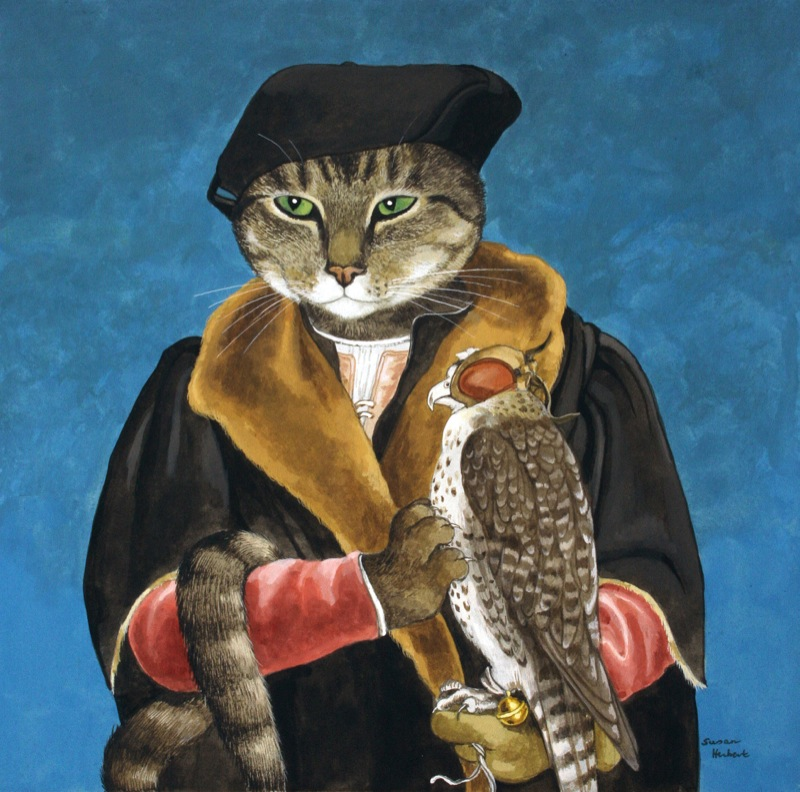
\includegraphics[scale=0.4]{cat-painting}%include full file path unless source file is in the same directory.
\caption{Robert Cheseman (Holbein)\cite{Herbert}}
\label{fig:Cat Lord}
\end{figure}

Also keep in mind:

\begin{enumerate} %start numbered list
  \item You should be mindful of the number of significant digits you use in your results.
  \item Use consistent units and suitable unit prefixes.
  \item When referring to equations, figures, tables, and appendices in your memo you must always capitalize E in equation F in figure, T in table, and A in appendix.
  \item To reference an equation from the manual don't say "according to Equation 8.25 in the manual". The correct way to do this is: "according to Equation 2 [X]”. Note Equation 2 is an equation in your memo and has its own number and [X] is the citation number in your reference section corresponding to the appropriate source.
  \item Table, figure, and equation titles: Tables get titles on top. Figures and equations get the title on the bottom.
  \item Tables, figures and equations must be part of the written text. That is you should put your table, figure, and equation right below the paragraph where they are first mentioned.
  \item Only include necessary data in tables that are related to the analysis of the experiment.
\end{enumerate}

\section*{Discussion Questions}
In this section, simply answer each question from the lab manual in order. It may be wise to number your responses. Some responses require equations - number your equations in the order they appear. Equation~\ref{Quadratic} displays the proper formatting; Equation~\ref{eq:Dirac} is a more complex example with a more traditional numbering scheme.

%this equation has a caption BELOW it
\begin{eqfloat}[!htb]
	\begin{equation*}
		x=\frac{-b\pm\sqrt{b^2-4ac}}{2a}
	\end{equation*}
\caption{The Quadratic Formula}
\label{Quadratic}
\end{eqfloat}
	
%this equation has no caption - the number is right-justified
\begin{equation}
	\label{eq:Dirac}
	\left (
  \beta mc^2 + c 
     \left ( 
         \sum_{n=1}^3 \alpha_n p_n 
     \right )
	\right )
	\psi(x,t)
	=
	i \hbar \dfrac{\partial \psi(x,t) }{\partial t}
\end{equation}

%note that the equation numbering auto-increments and the in-line references update accordingly. Tables and figures behave the same way.

\section*{Conclusion}
This section is where the author interprets the Results and attempts to persuade the audience. It should reflect the form and topics discussed in the Introduction. If the Introduction is laid out in an A, B, C format, then the Conclusion should be as well. Recommendations may include recommendations for continued study, ways to improve data collection and interpretation, or any other thoughts governing future study that the author may have. Bibliography (or References).

\section*{Bibliography}
The Bibliography should reference all material the author used to produce the publication. This includes all figures used that the author did not directly create, information gained from the Internet, books, magazines, etc. Permission must be gained from the author of any source with a copy write that is to be included in the
publication. All references cited in the paper are placed here in the format recommended by the journal or conference to which the paper will be submitted.
You may use any format for the bibliography that you like as long as it is consistently followed. There are several standards to choose from, such as MLA.

%A pure LaTeX bibliography 
\begin{thebibliography}{9}

	\bibitem{Herbert}
	  Herbert, S.,\emph{Robert Cheseman (Holbein).}
	  Chris Beetles Gallery, London, England, www.chrisbeetles.com/gallery/animals/cats/robert-cheseman-holbein.html. Accessed 8 Nov. 2018.
	  
	\bibitem{Stutts}
	  Stutts, D.S., \emph{Mechanical Engineering Systems Laboratory.}
	  Department of Mechanical and Aerospace Engineering, Missouri University of Science and Technology, 25 Jan. 2019. 142-146.
	  
	\bibitem{Vigen}
	  Vigen, T., \emph{15 Insane Things That Correlate With Each Other.}
	  Spurious Correlations, tylervigen.com/spurious-correlations. Accessed 8 Nov. 2018.

\end{thebibliography}

\newpage %force a new page
\section*{Appendix A - \textnormal{Appendices}}
The Appendix should include any work to expand on the results that did not directly fit into the Body. This includes program source code, long mathematical derivations, answers to lab manual questions, and other highly detailed explanations. There may be any number of appendices, and they are designated: \textbf{Appendix A —} \textit{Appendix A Title}, \textbf{Appendix B –} \textit{Appendix B Title}, etc.

\newpage 
\section*{Appendix B: Usage}
If you run into problems using this template, please first refer to the accompanying documentation named Memo-Template-Commentary.

\end{document}